\documentclass[8pt, landscape, a4paper]{extarticle}

% --- 核心宏包 ---
\usepackage[UTF8]{ctex}
\usepackage[margin=0.8cm, top=1cm, bottom=1.3cm]{geometry}
\usepackage{multicol}
\usepackage{xcolor}
\usepackage{tcolorbox}
\usepackage{enumitem}
\usepackage{amsmath}
\usepackage{amssymb}
\usepackage{fontspec}
\usepackage{tikz}
\usetikzlibrary{arrows.meta, shapes}

% --- 去掉页码 ---
\pagestyle{empty}

% --- 颜色定义 (Red 主题) ---
\definecolor{headerblue}{RGB}{192, 57, 43}     % Red
\definecolor{navcolor}{RGB}{211, 84, 0}        % 导航橙
\definecolor{intuitioncolor}{RGB}{41, 128, 185}% 直觉蓝
\definecolor{accentcolor}{RGB}{243, 156, 18}   % 强调黄
\definecolor{section2}{RGB}{22, 160, 133}      % 绿色
\definecolor{dividergray}{RGB}{220, 220, 220}

% --- 全局设置 ---
\setlength{\parindent}{0pt}
\setlength{\columnsep}{0.4cm} 
\linespread{1.1} 

% --- 列表样式 ---
\setlist[itemize]{leftmargin=1.2em, nosep, itemsep=2pt, topsep=2pt, label=$\textcolor{headerblue}{\vcenter{\hbox{\tiny$\bullet$}}}$ }
\setlist[description]{leftmargin=0.2em, style=sameline, nosep, itemsep=2pt, font=\bfseries}

% --- Box 样式 ---
\newtcolorbox{mybox}[2][]{%
  colback=white,
  colframe=#2,
  coltitle=white,
  boxrule=1pt,             
  arc=2mm,                 
  left=4pt, right=4pt, top=3pt, bottom=3pt, 
  toptitle=3pt, bottomtitle=3pt, 
  fonttitle=\bfseries\sffamily\large,
  title={#1},
  after skip=5pt          
}

% --- 自定义命令 ---
\newcommand{\subt}[1]{{\vspace{2pt}\textbf{\large \textcolor{black}{#1}}}}

\newcommand{\boxdesc}[1]{%
    \textit{\small \textcolor{gray}{#1}}%
    \par\vspace{2pt}%
    {\color{dividergray}\hrule height 0.5pt}%
    \vspace{2pt}%
}

\newcommand{\sepline}{%
    \par \vspace{3pt}%
    {\color{dividergray}\hrule height 0.5pt}%
    \par \vspace{3pt}%
}

% 公式间距
\setlength{\abovedisplayskip}{3pt}
\setlength{\belowdisplayskip}{3pt}

\begin{document}

% --- 页眉 ---
\begin{center}
    {\Huge \textbf{\sffamily \textcolor{headerblue}{博弈论 Game Theory Cheat Sheet}}} \\
    \vspace{0.2cm}
    {\large \texttt{Strategic Decision Making: From Nash Equilibrium to Mechanism Design}}
\end{center}

% --- 开始四栏布局 ---
\begin{multicols*}{4}

% === 第一栏 ===

\begin{mybox}[️ 场景导航 (Use Cases)]{navcolor}
    \boxdesc{遇到什么问题 $\to$ 用什么工具}
    \begin{itemize}[itemsep=2pt]
        \item \textbf{多方竞争/合作} $\to$ 纳什均衡 (Nash Eq)
        \item \textbf{拍卖/广告竞价} $\to$ 机制设计 (VCG)
        \item \textbf{对抗生成网络} $\to$ 极小极大 (Minimax)
        \item \textbf{区块链共识} $\to$ 拜占庭容错 (BFT)
        \item \textbf{资源调度} $\to$ 合作博弈 (Shapley Value)
        \item \textbf{演化策略} $\to$ 演化博弈 (ESS)
    \end{itemize}
\end{mybox}

\begin{mybox}[1. 基础定义 (Foundations)]{headerblue}
    \boxdesc{玩家、策略与收益}
    
    \subt{博弈三要素}
    \begin{itemize}
        \item \textbf{Players ($N$)}: 参与者集合。
        \item \textbf{Strategies ($S_i$)}: 每个玩家的可选动作。
        \item \textbf{Payoffs ($u_i$)}: 收益函数 $u_i(s_1, \dots, s_n)$。
    \end{itemize}
    \sepline
    
    \subt{纳什均衡 (Nash Equilibrium)}
    策略组合 $s^*$,使得没有任何玩家可以通过\textbf{单方面}改变策略来获益。
    $$ u_i(s_i^*, s_{-i}^*) \ge u_i(s_i, s_{-i}^*) \quad \forall s_i \in S_i $$
    \textit{含义: 稳定的僵局,没人想动。}
\end{mybox}

\begin{mybox}[2. 经典模型 (Classics)]{headerblue}
    \boxdesc{人性的囚笼}
    
    \subt{囚徒困境 (Prisoner's Dilemma)}
    \begin{center}
    \begin{tabular}{c|c|c}
         & 抵赖 & 坦白 \\ \hline
        抵赖 & (-1, -1) & (-3, 0) \\ \hline
        坦白 & (0, -3) & \textbf{(-2, -2)}
    \end{tabular}
    \end{center}
    \textit{结论: 个体理性导致集体非理性 (帕累托次优)。}
    \sepline
    
    \subt{协调博弈 (Coordination)}
    (左, 左) 和 (右, 右) 都是均衡。
    \textit{问题: 如何达成共识?(Focal Point)}
    \sepline
    
    \subt{零和博弈 (Zero-Sum)}
    一方收益 = 另一方损失。$\sum u_i = 0$。
    \textit{解法: Minimax 定理。}
\end{mybox}

\columnbreak

% === 第二栏 ===

\begin{mybox}[3. 混合策略 (Mixed Strategy)]{headerblue}
    \boxdesc{随机应变}
    
    \subt{定义}
    玩家以概率分布 $\sigma_i$ 选择策略。
    \textit{例: 石头剪刀布,最优策略是 (1/3, 1/3, 1/3)。}
    \sepline
    
    \subt{纳什存在性定理}
    任何有限博弈至少存在一个混合策略纳什均衡。
    \textit{证明用到不动点定理 (Brouwer)。}
\end{mybox}

\begin{mybox}[4. 动态博弈 (Dynamic)]{headerblue}
    \boxdesc{时间与顺序}
    
    \subt{扩展式 (Extensive Form)}
    博弈树 (Game Tree)。
    \begin{itemize}
        \item \textbf{信息集}: 玩家不知道自己在树的哪个节点 (不完全信息)。
    \end{itemize}
    \sepline
    
    \subt{子博弈精炼均衡 (SPE)}
    在博弈树的每一个子树上都是纳什均衡。
    \textit{解法: 逆向归纳法 (Backward Induction)。}
    \textit{应用: 排除不可信的威胁。}
\end{mybox}

\begin{mybox}[5. 机制设计 (Mechanism Design)]{headerblue}
    \boxdesc{反向博弈论:制定规则}
    
    \subt{目标}
    设计规则 (游戏),使得自私玩家的均衡结果符合整体利益 (如社会福利最大化)。
    \sepline
    
    \subt{VCG 机制}
    支付 = 给他人造成的“负外部性”。
    \textit{特性: 说真话是占优策略 (Truthful)。}
    \textit{应用: 谷歌/百度广告竞价 (GSP 是 VCG 的变体)。}
\end{mybox}

\columnbreak

% === 第三栏 ===

\begin{mybox}[6. 合作博弈 (Cooperative)]{headerblue}
    \boxdesc{结盟与分赃}
    
    \subt{夏普利值 (Shapley Value)}
    公平分配收益的唯一解。
    $$ \phi_i(v) = \sum_{S \subseteq N \setminus \{i\}} \frac{|S|!(n-|S|-1)!}{n!} (v(S \cup \{i\}) - v(S)) $$
    \textit{直觉: 贡献越大,拿得越多 (边际贡献的期望)。}
    \textit{应用: 机器学习特征重要性解释 (SHAP)。}
\end{mybox}

\begin{mybox}[7. 演化博弈 (Evolutionary)]{headerblue}
    \boxdesc{适者生存}
    
    \subt{演化稳定策略 (ESS)}
    如果种群都采用策略 $S$,突变策略 $T$ 无法入侵。
    $$ u(S, S) > u(T, S) \quad \text{或者} \quad u(S, S) = u(T, S) \text{且} u(S, T) > u(T, T) $$
    \textit{应用: 生物学 (鹰鸽博弈),算法优化。}
\end{mybox}

\begin{mybox}[8. Python / Gambit 实战]{headerblue}
    \boxdesc{代码工具箱}
    \begin{itemize}
        \item \textbf{Nashpy}:
        \texttt{game = nashpy.Game(A, B)}
        \texttt{game.support\_enumeration()}
        \item \textbf{Axelrod}: 囚徒困境锦标赛模拟。
        \item \textbf{OpenSpiel}: DeepMind 的强化学习博弈库。
    \end{itemize}
\end{mybox}

\columnbreak

% === 第四栏 ===

\begin{mybox}[9. 高阶前沿 (Advanced)]{headerblue}
    \boxdesc{复杂系统}
    
    \subt{算法博弈论 (AGT)}
    关注均衡的计算复杂度 (PPAD Complete) 和效率损失。
    \textbf{无政府代价 (PoA)}:
    $$ PoA = \frac{\text{最差均衡的社会福利}}{\text{全局最优社会福利}} $$
    \textit{例: 交通拥堵 (Braess 悖论)。}
    \sepline
    
    \subt{平均场博弈 (Mean Field)}
    玩家数量 $N \to \infty$。个体只与“平均分布”交互。
    \textit{应用: 鱼群模拟,高频交易。}
\end{mybox}

\vspace*{\fill}

\begin{mybox}[ 核心直觉 (Intuition)]{intuitioncolor}
    \boxdesc{“预测对手的预测。”}
    
    % TikZ 矢量图: 极小极大 (Minimax) 或 纳什均衡点
    \begin{center}
    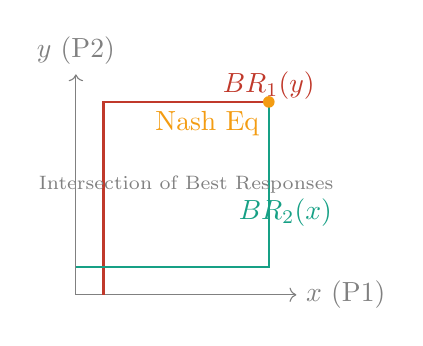
\begin{tikzpicture}[scale=0.7]
        % 坐标轴
        \draw[->, gray] (0,0) -- (4,0) node[right] {$x$ (P1)};
        \draw[->, gray] (0,0) -- (0,4) node[above] {$y$ (P2)};
        
        % 反应函数 (Best Response)
        \draw[thick, headerblue] (0.5, 0) -- (0.5, 3.5) -- (3.5, 3.5);
        \node[headerblue] at (3.5, 3.8) {$BR_1(y)$};
        
        \draw[thick, section2] (0, 0.5) -- (3.5, 0.5) -- (3.5, 3.5);
        \node[section2] at (3.8, 1.5) {$BR_2(x)$};
        
        % 均衡点
        \fill[accentcolor] (3.5, 3.5) circle (3pt);
        \node[below left, accentcolor] at (3.5, 3.5) {Nash Eq};
        
        % 解释
        \node[font=\scriptsize, gray] at (2, 2) {Intersection of Best Responses};
    \end{tikzpicture}
    \end{center}

    \hspace{1em}博弈论不是教你怎么赢,而是教你在\textbf{理性对手}面前如何不输。
    \vspace{4pt}
    
    \subt{三大核心视角}
    \begin{itemize}[itemsep=4pt]
        \item \textbf{均衡即稳定}: 
        物理系统趋向于能量最低,博弈系统趋向于纳什均衡。一旦达到均衡,系统就锁死了,除非改变规则。
        
        \item \textbf{承诺即力量}: 
        在动态博弈中,限制自己的选择权 (如破釜沉舟) 反而能增加谈判筹码。不可信的威胁是无效的。
        
        \item \textbf{规则优于策略}: 
        如果你不喜欢均衡的结果 (如内卷),不要试图改变玩家的策略 (说教),而要改变游戏的规则 (机制设计)。
    \end{itemize}
    
    \vspace{6pt}
    \centering\textit{\footnotesize 每一个选择,都是对未来世界的一次投票。}
\end{mybox}

\end{multicols*}

\end{document}
